\section{WC 19/5/25}

\subsection*{Overview:}
Back from exams and feeling refreshed I first to tackling some stubborn bugs I had yet to iron out

\subsection*{Achievements, Thoughts and Ideas:}

As I sat down to begin coding I very quickly found that this time away to gather a 'fresh point of view' had been incredibly beneficial. Writing my dashboard code from the ground up I solved my overflowing layout challenges and produced an adaptive layout that scaled itself to 9 differing sizes depending on the type of screen my webapp is viewed on. Using a technique known as "breakpoints" my code would analyse the width of the screen to determine 1 of 3 'block' layouts (mobile, tablet, desktop) and then compare the height of the screen to intelligently add less crucial but aesthetically pleasing decorators (such as my welcome bar and note stats). Please see below for some examples of this in action for a variety of screen sizes.

\begin{figure}[H]
    \centering
    \begin{minipage}[b]{0.48\textwidth}
        \centering
        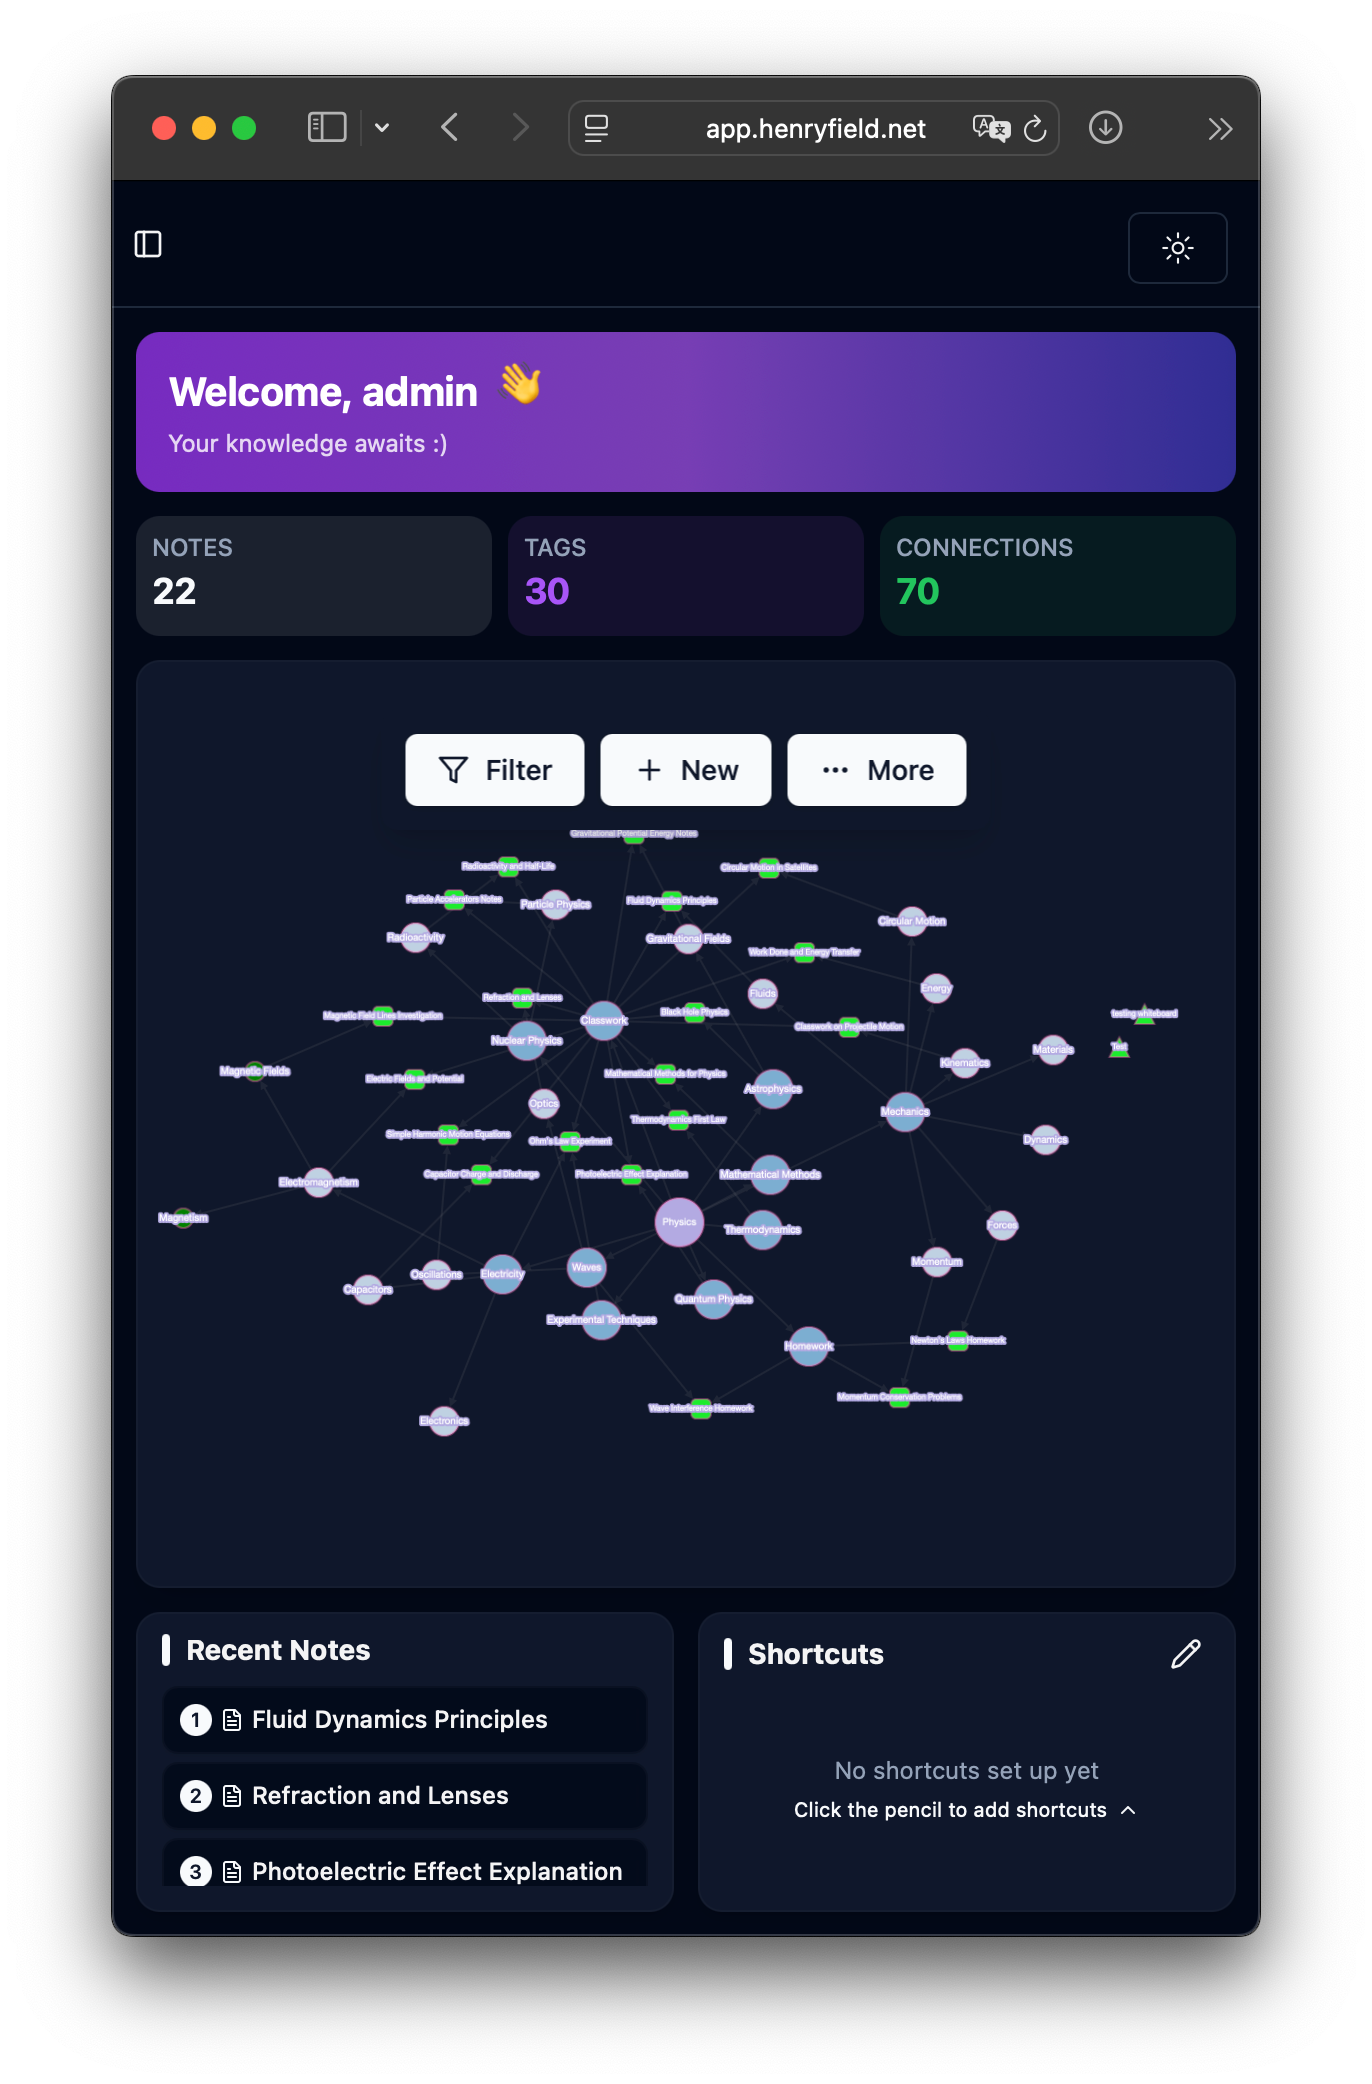
\includegraphics[width=\textwidth]{Diary/29_WC_19-5-25/media/tallMobile.png}
        \caption{Tall Mobile view}
    \end{minipage}
    \hfill
    \begin{minipage}[b]{0.48\textwidth}
        \centering
        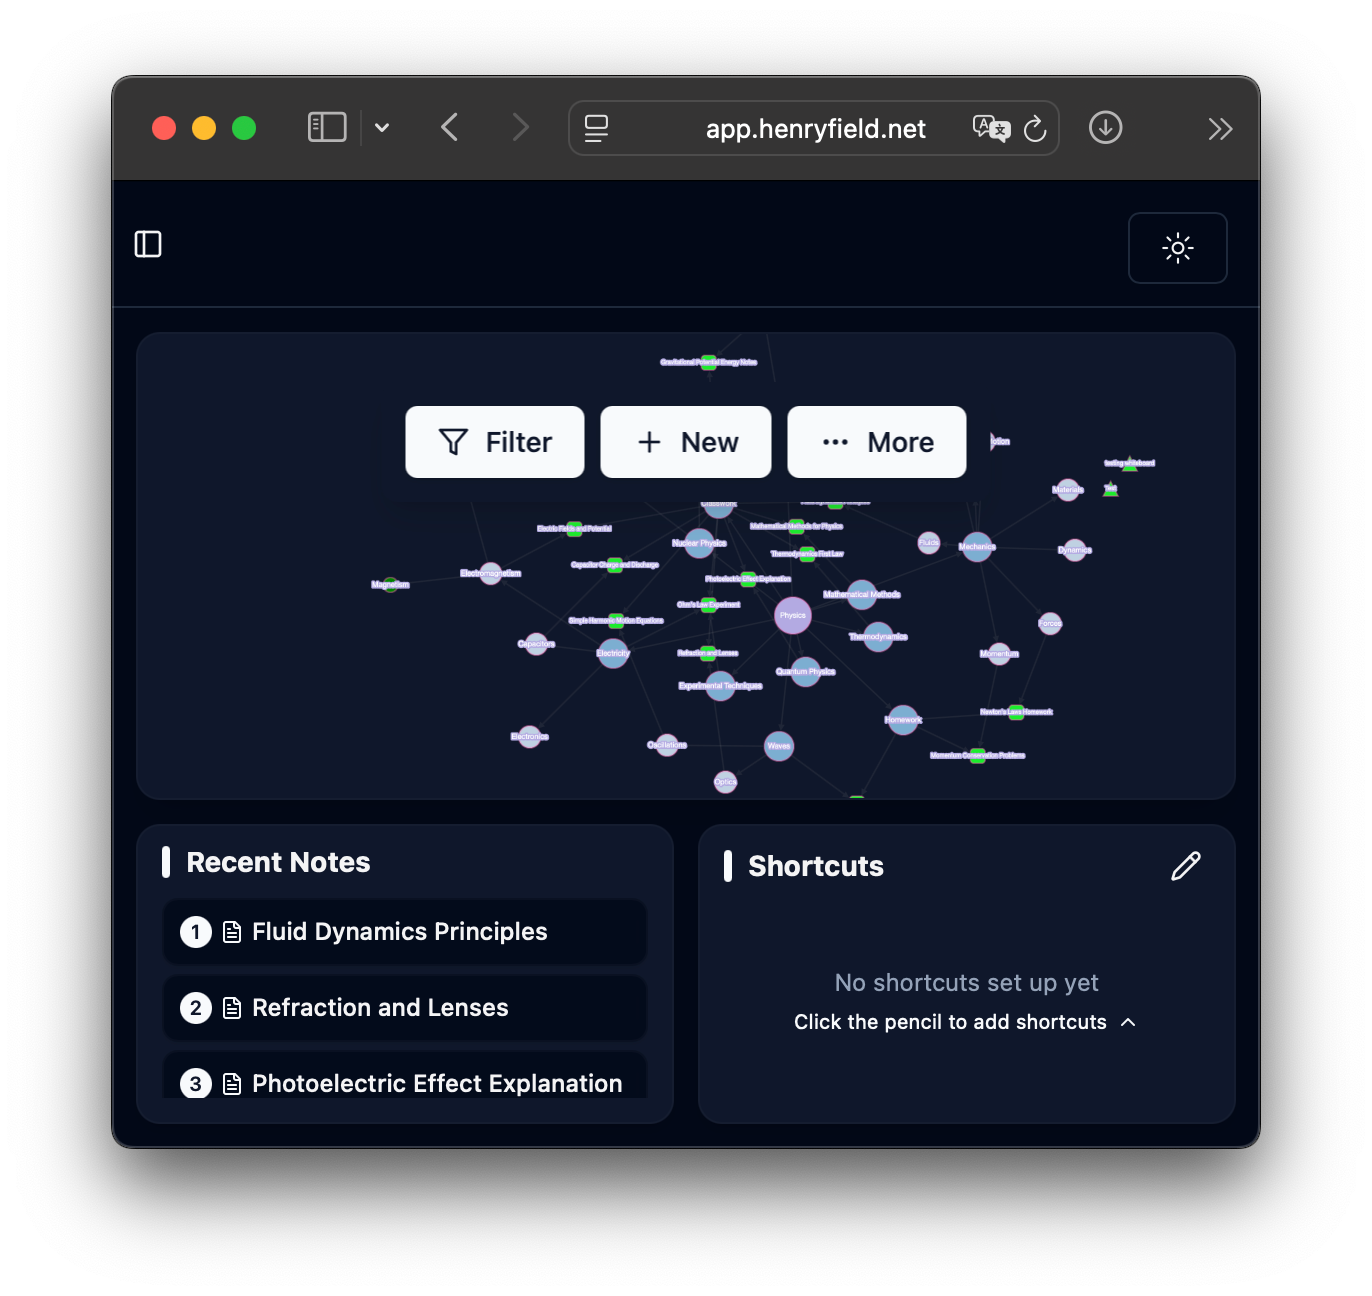
\includegraphics[width=\textwidth]{Diary/29_WC_19-5-25/media/shortTablet.png}
        \caption{Short Tablet view}
    \end{minipage}
\end{figure}

\begin{figure}[H]
    \centering
   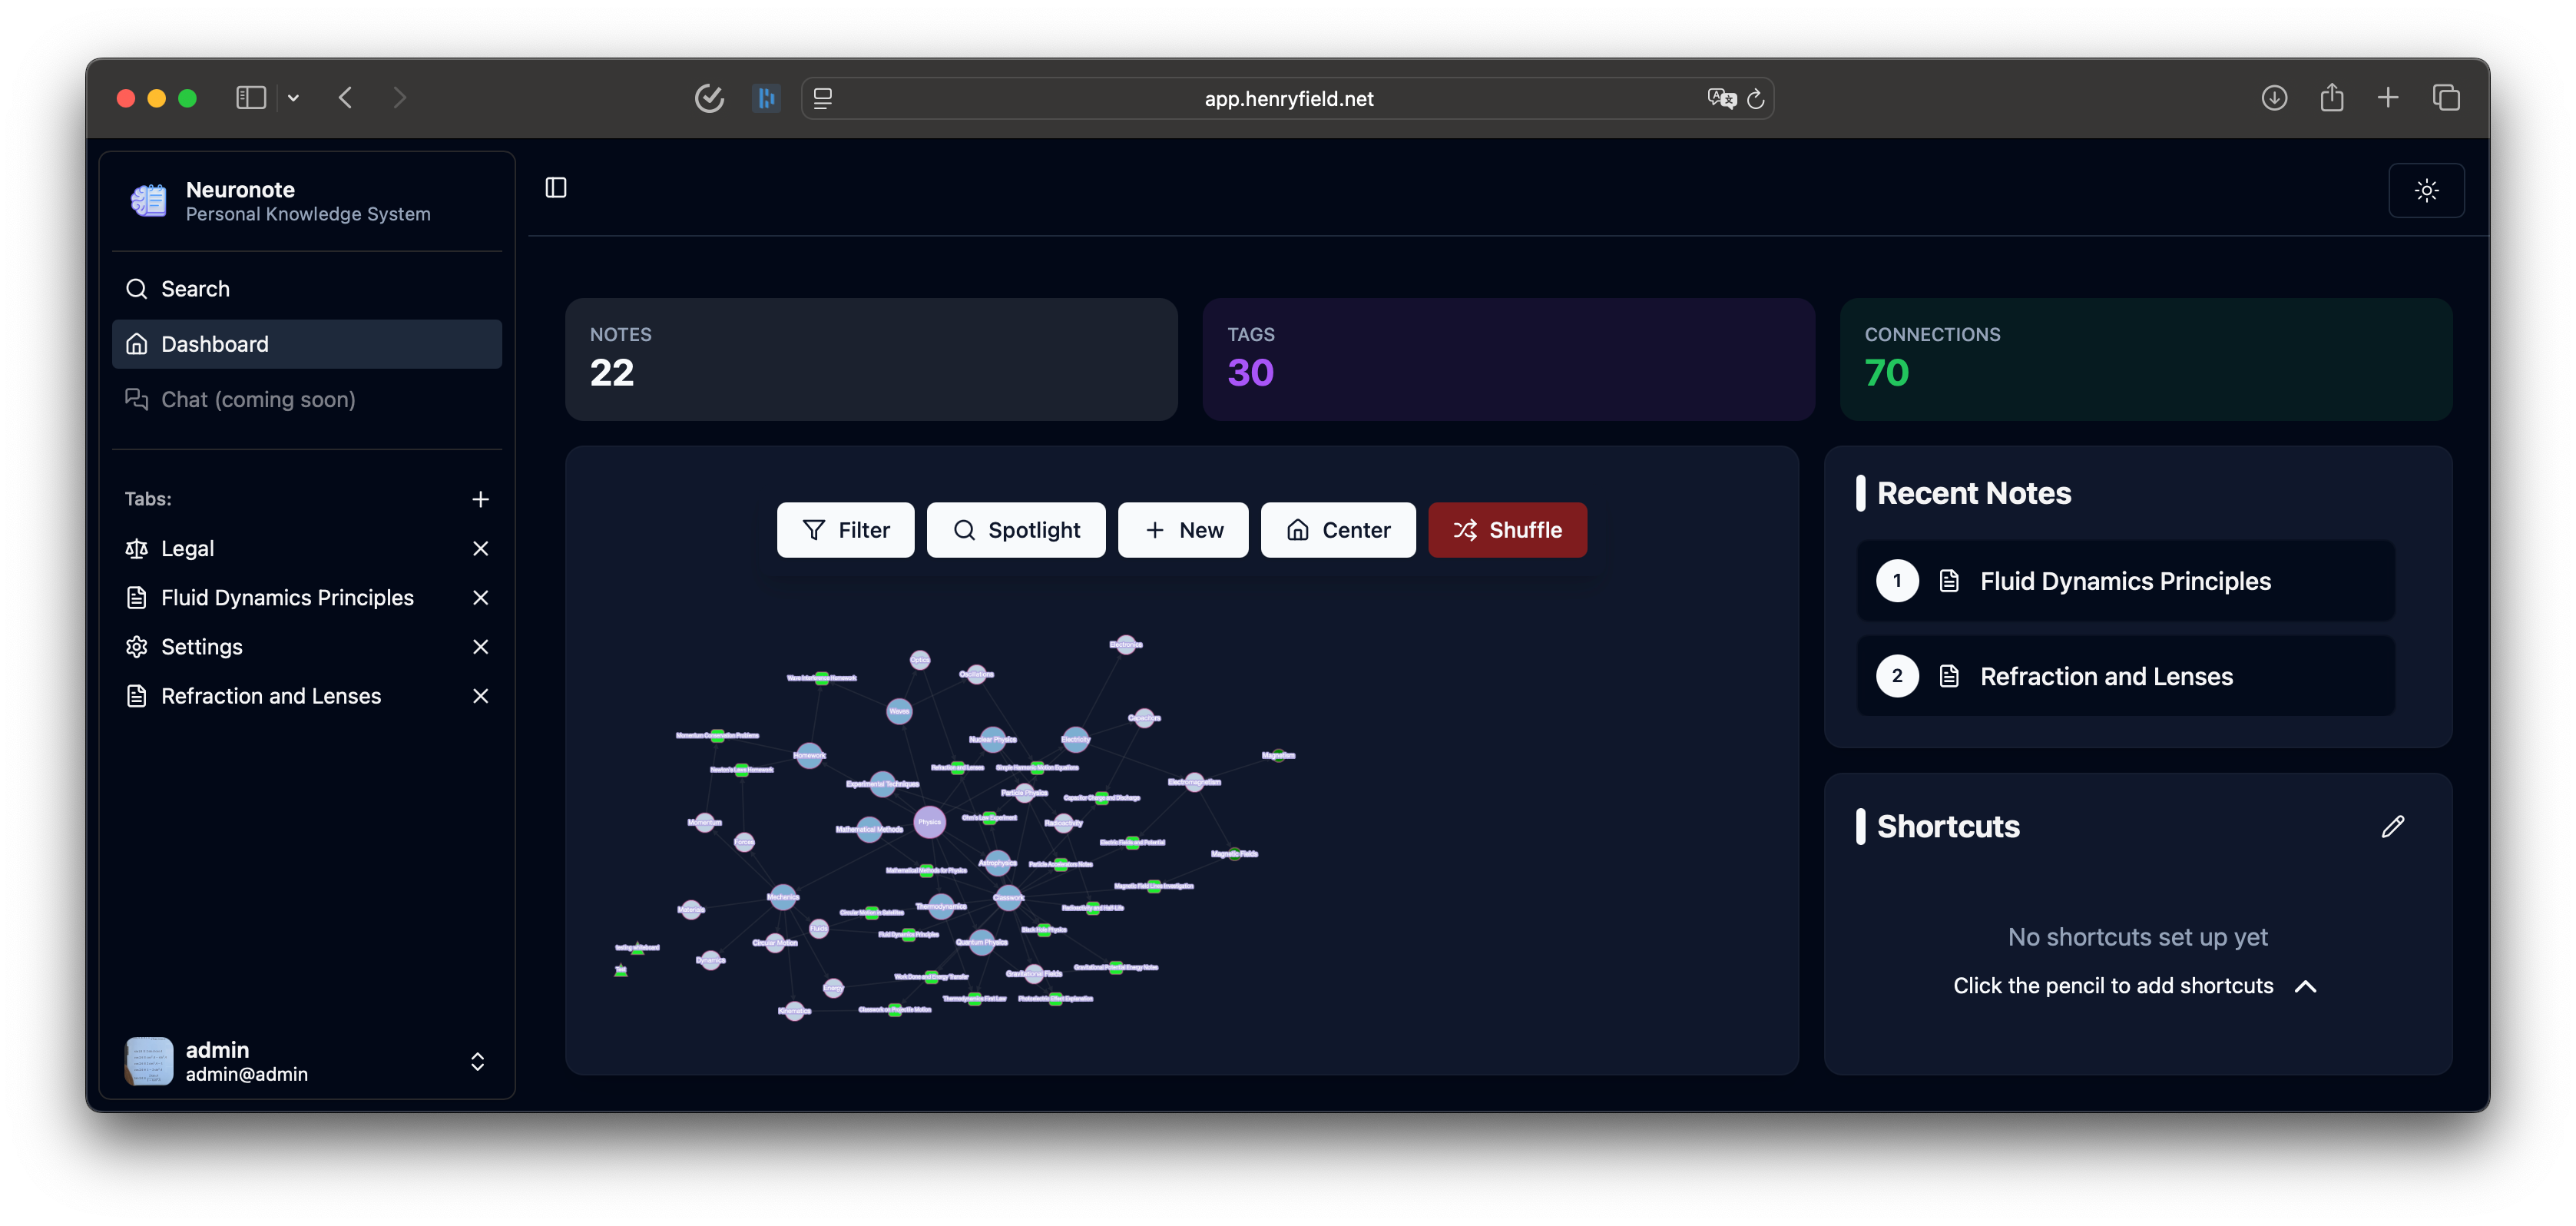
\includegraphics{Diary/29_WC_19-5-25/media/mediumDesktop.png}
    \caption{Medium Desktop view}
\end{figure}

Whilst working on the dashboard I spotted some confirmation dialogues and text prompts that had remained unchanged from the very start of my prototyping. These user prompts use the default browser input methods which whilst reliable and cross platform (working on most devices) aren't very visually appealing and break my design style. Additionally id experienced a couple of browser / device freezes If a user navigated to a different app as the popup appeared. I replaced the bowser generic popups with my own custom design styled in the same way as the rest of my ui. By making these into generic functions I could call system wide and I have replaced all uses of the prior (white) prompts for my newly updated custom alternative.

\begin{figure}[H]
    \centering
    \begin{minipage}[b]{0.48\textwidth}
        \centering
        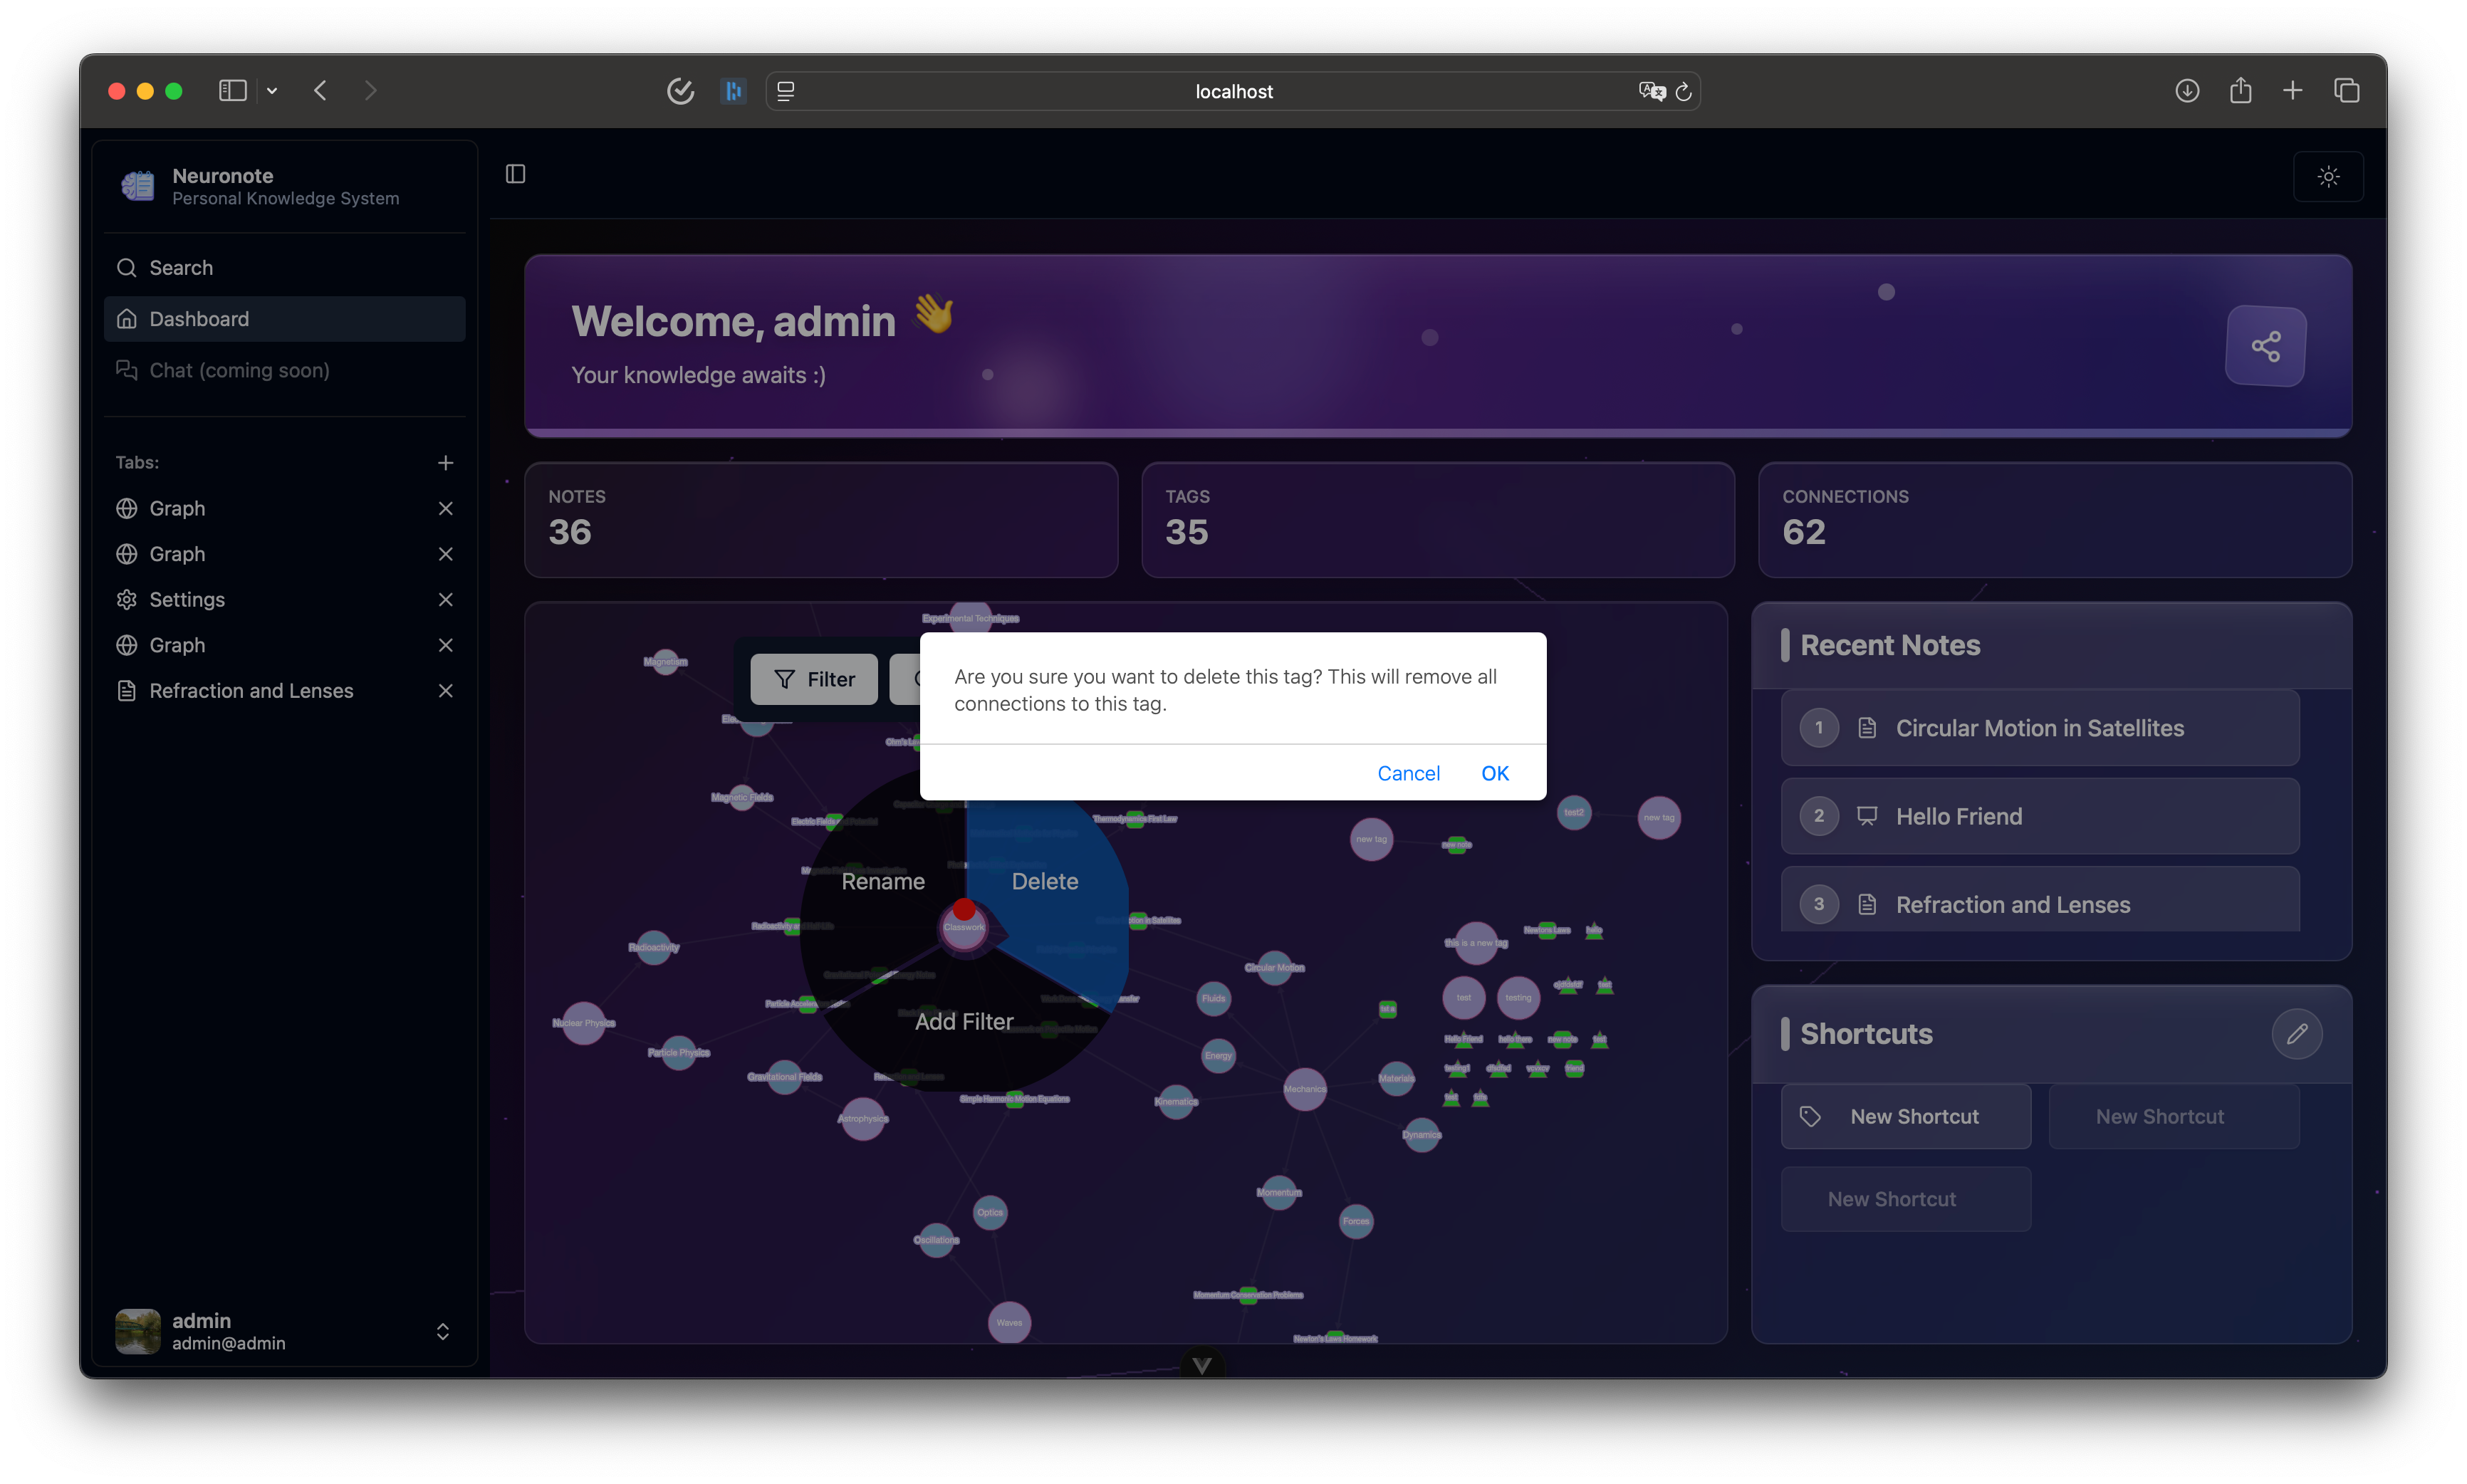
\includegraphics[width=\textwidth]{Diary/29_WC_19-5-25/media/oldDialogue.png}
        \caption{Old generic browser prompts}
    \end{minipage}
    \hfill
    \begin{minipage}[b]{0.48\textwidth}
        \centering
        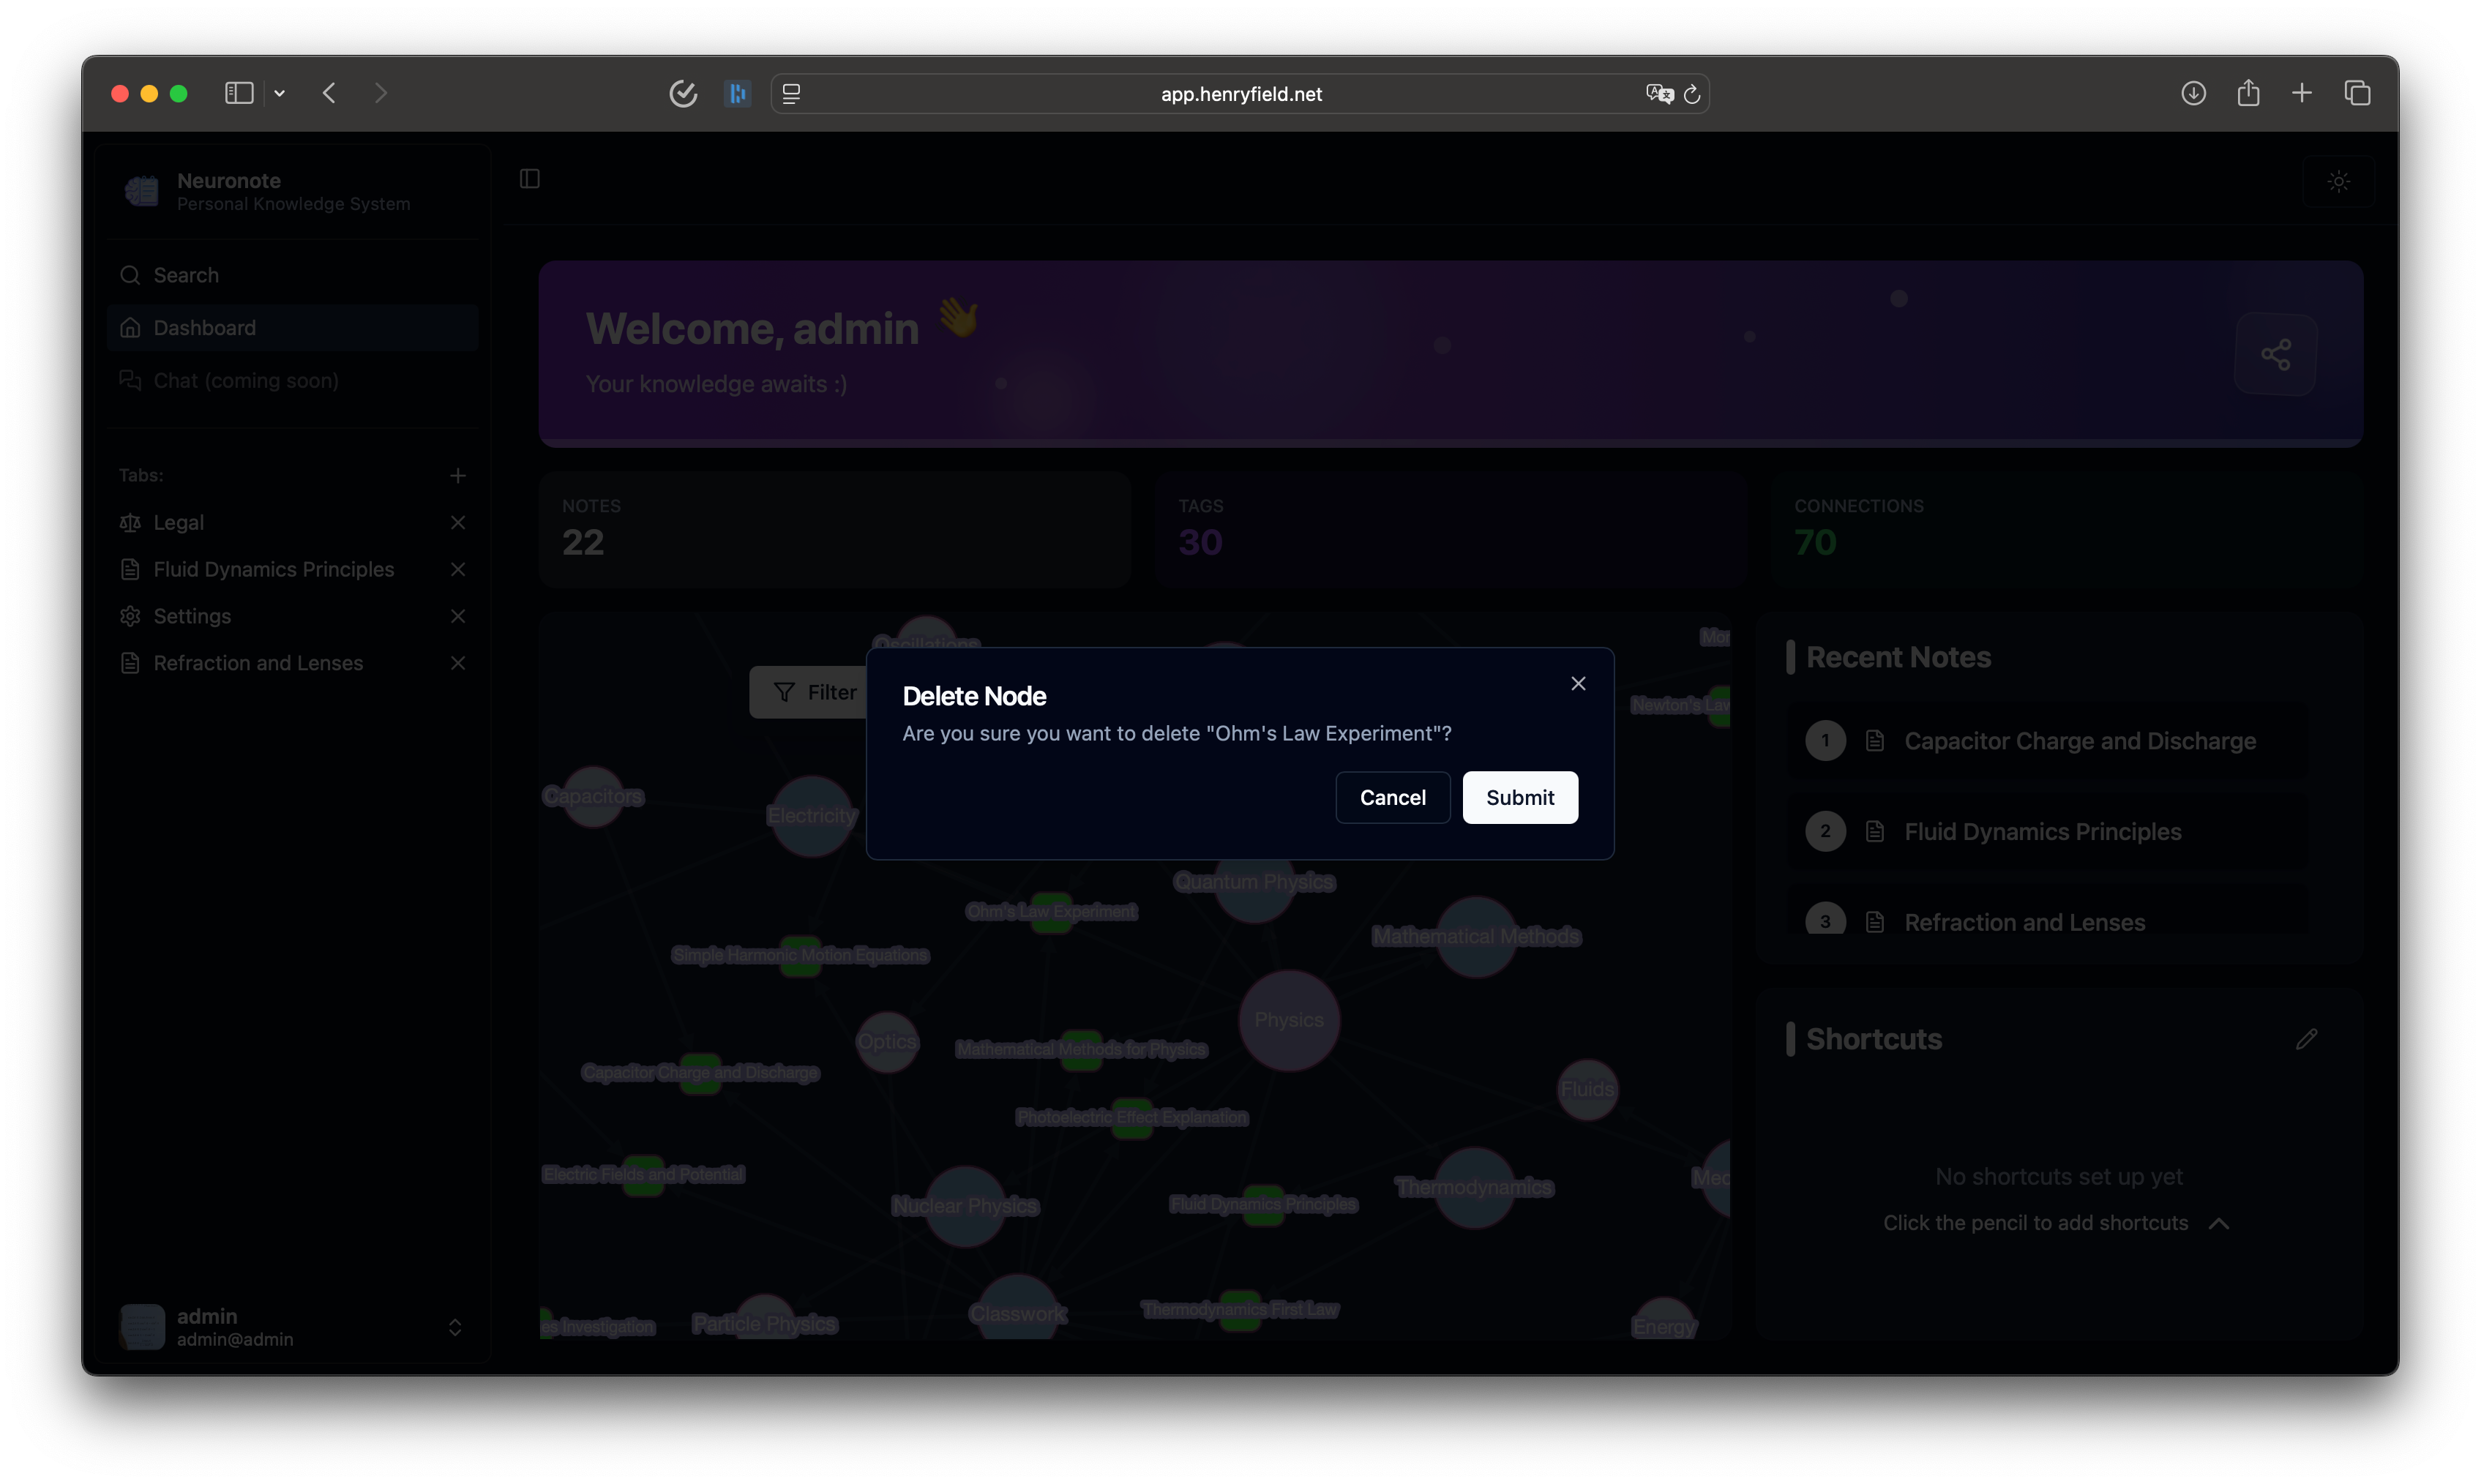
\includegraphics[width=\textwidth]{Diary/29_WC_19-5-25/media/newDialogue.png}
        \caption{New custom prompts (with custom input fields)}
    \end{minipage}
\end{figure}

Once I started using this new system I found a very niche bug in which pressing escape to cancel the dialogue whilst in full screen on safari on a MacBook would cause my device to freeze, I soon found a solution which eliminated these issues

A friend reported an instance of building up some connections  whilst in a highly filtered view, and upon leaving (and entering the general view) finding multiple lines / connections being displayed for each connection he made. After some investigating I found that the data being stored was fully correct (only having the one connection he added) but that I had a visual caching bug in which each time he exited a filtered view the prior connections displayed would not be taken account of when the system aimed to show the user all connections that existed between notes.

On mobile I had found a bug in which navigating the whiteboard (view multi finger pans and zooms) could trigger the current tool to rapidly switch between text and drawing which (while technically correct based on user intent) was causing performance issues and stuttering, by limiting the number of times this could be changed per second to 2 these issues were solved

A different user reported facing issues uploading images to her notes, upon investigation however it seems they lost internet connection midway through uploading the image (which cannot be helped) however this did teach me a valuable lesson in ensuring the user is shown a clear error message when network issues such as this occur and I have now implemented these.

Whilst I was at work improving my dashboard I also spent some time making my legal and settings pages more accessible to those on smaller screens / mobile devices. I added dropdown menus instead of static buttons to select the relevant pages and tuned the content of subsections to be more easily readable

My main challenge this week was to produce a guided tour for my users to navigate around my interface for the first time and learn all of my software's core functionality. During the holiday I did some research into \nameref{research:ShepardJS} and implemented my findings to produce a tour as can be seen on the right. I recommend reading through that research as it showcases the though process i folloed when designing my user tour. I also ensured it was possible for users to access the tour again for a 'quick refresher' by selecting the dedicated button in the user dropdown

\begin{figure}[H]
    \centering
    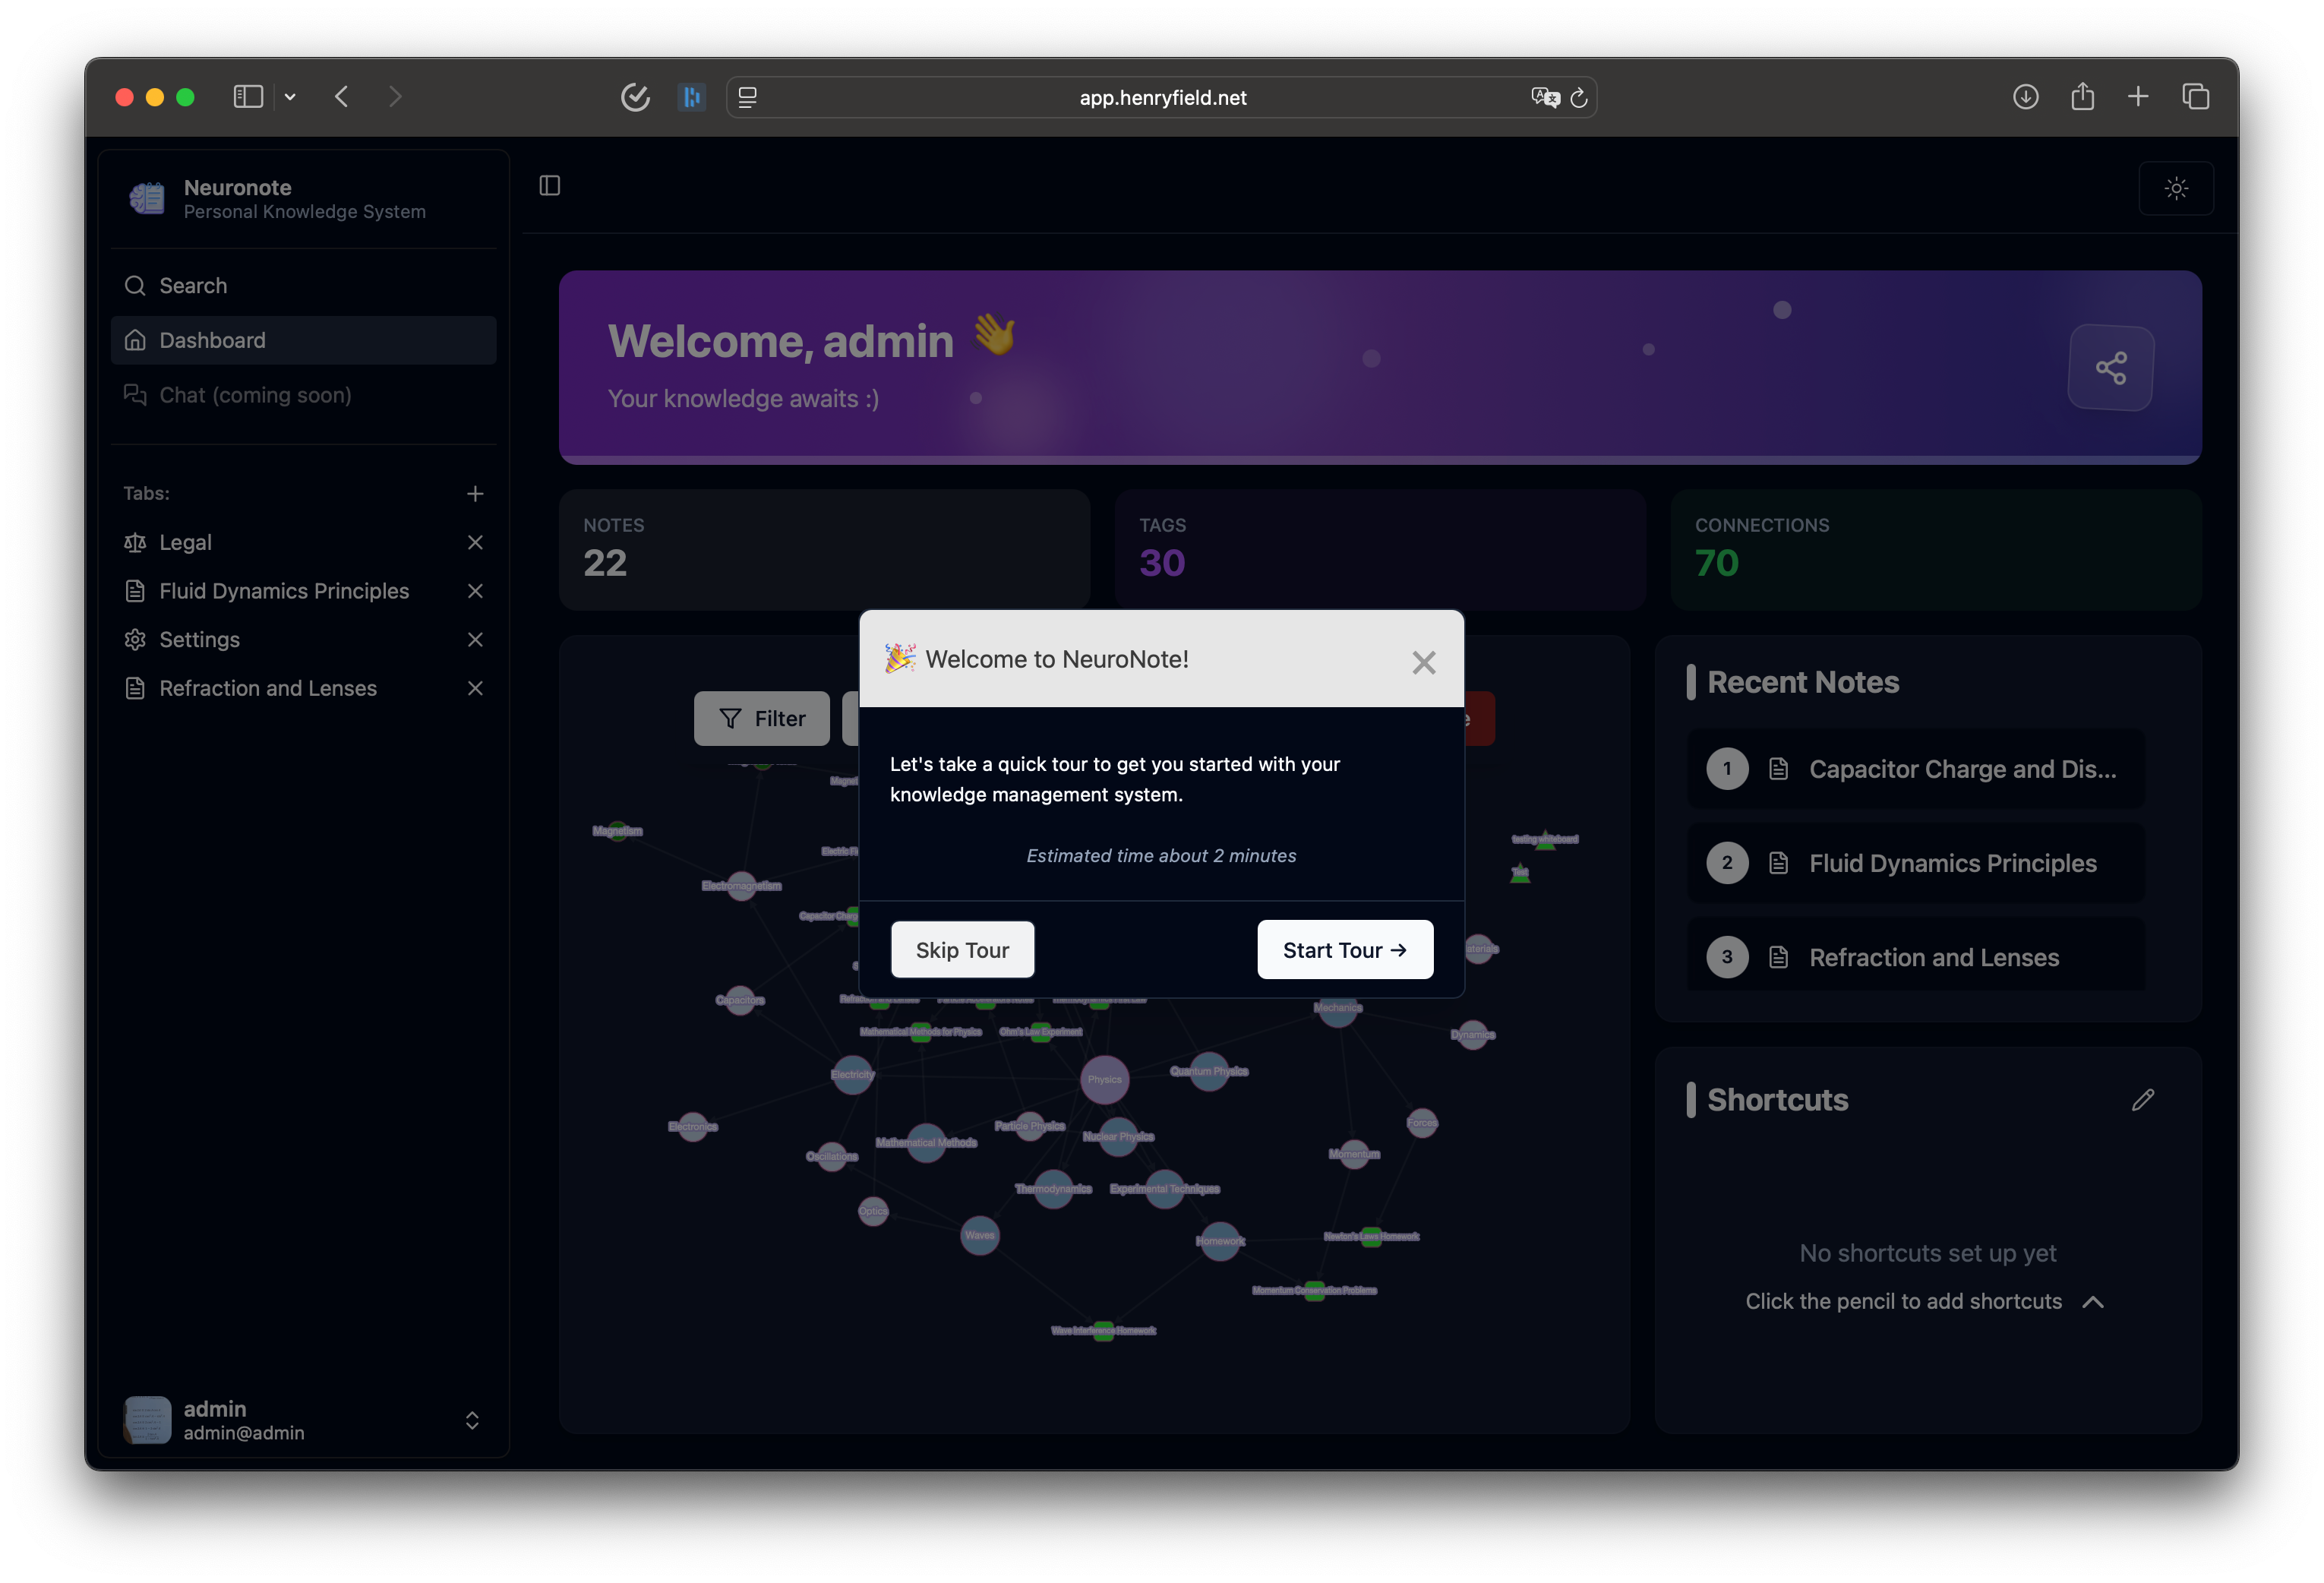
\includegraphics[width=0.8\linewidth]{Diary/29_WC_19-5-25/media/tourStart.png}
    \caption{New user tour start screen}
    \label{fig:user_tour}
\end{figure}

\begin{figure}[H]
    \centering
    \begin{minipage}[b]{0.48\textwidth}
        \centering
        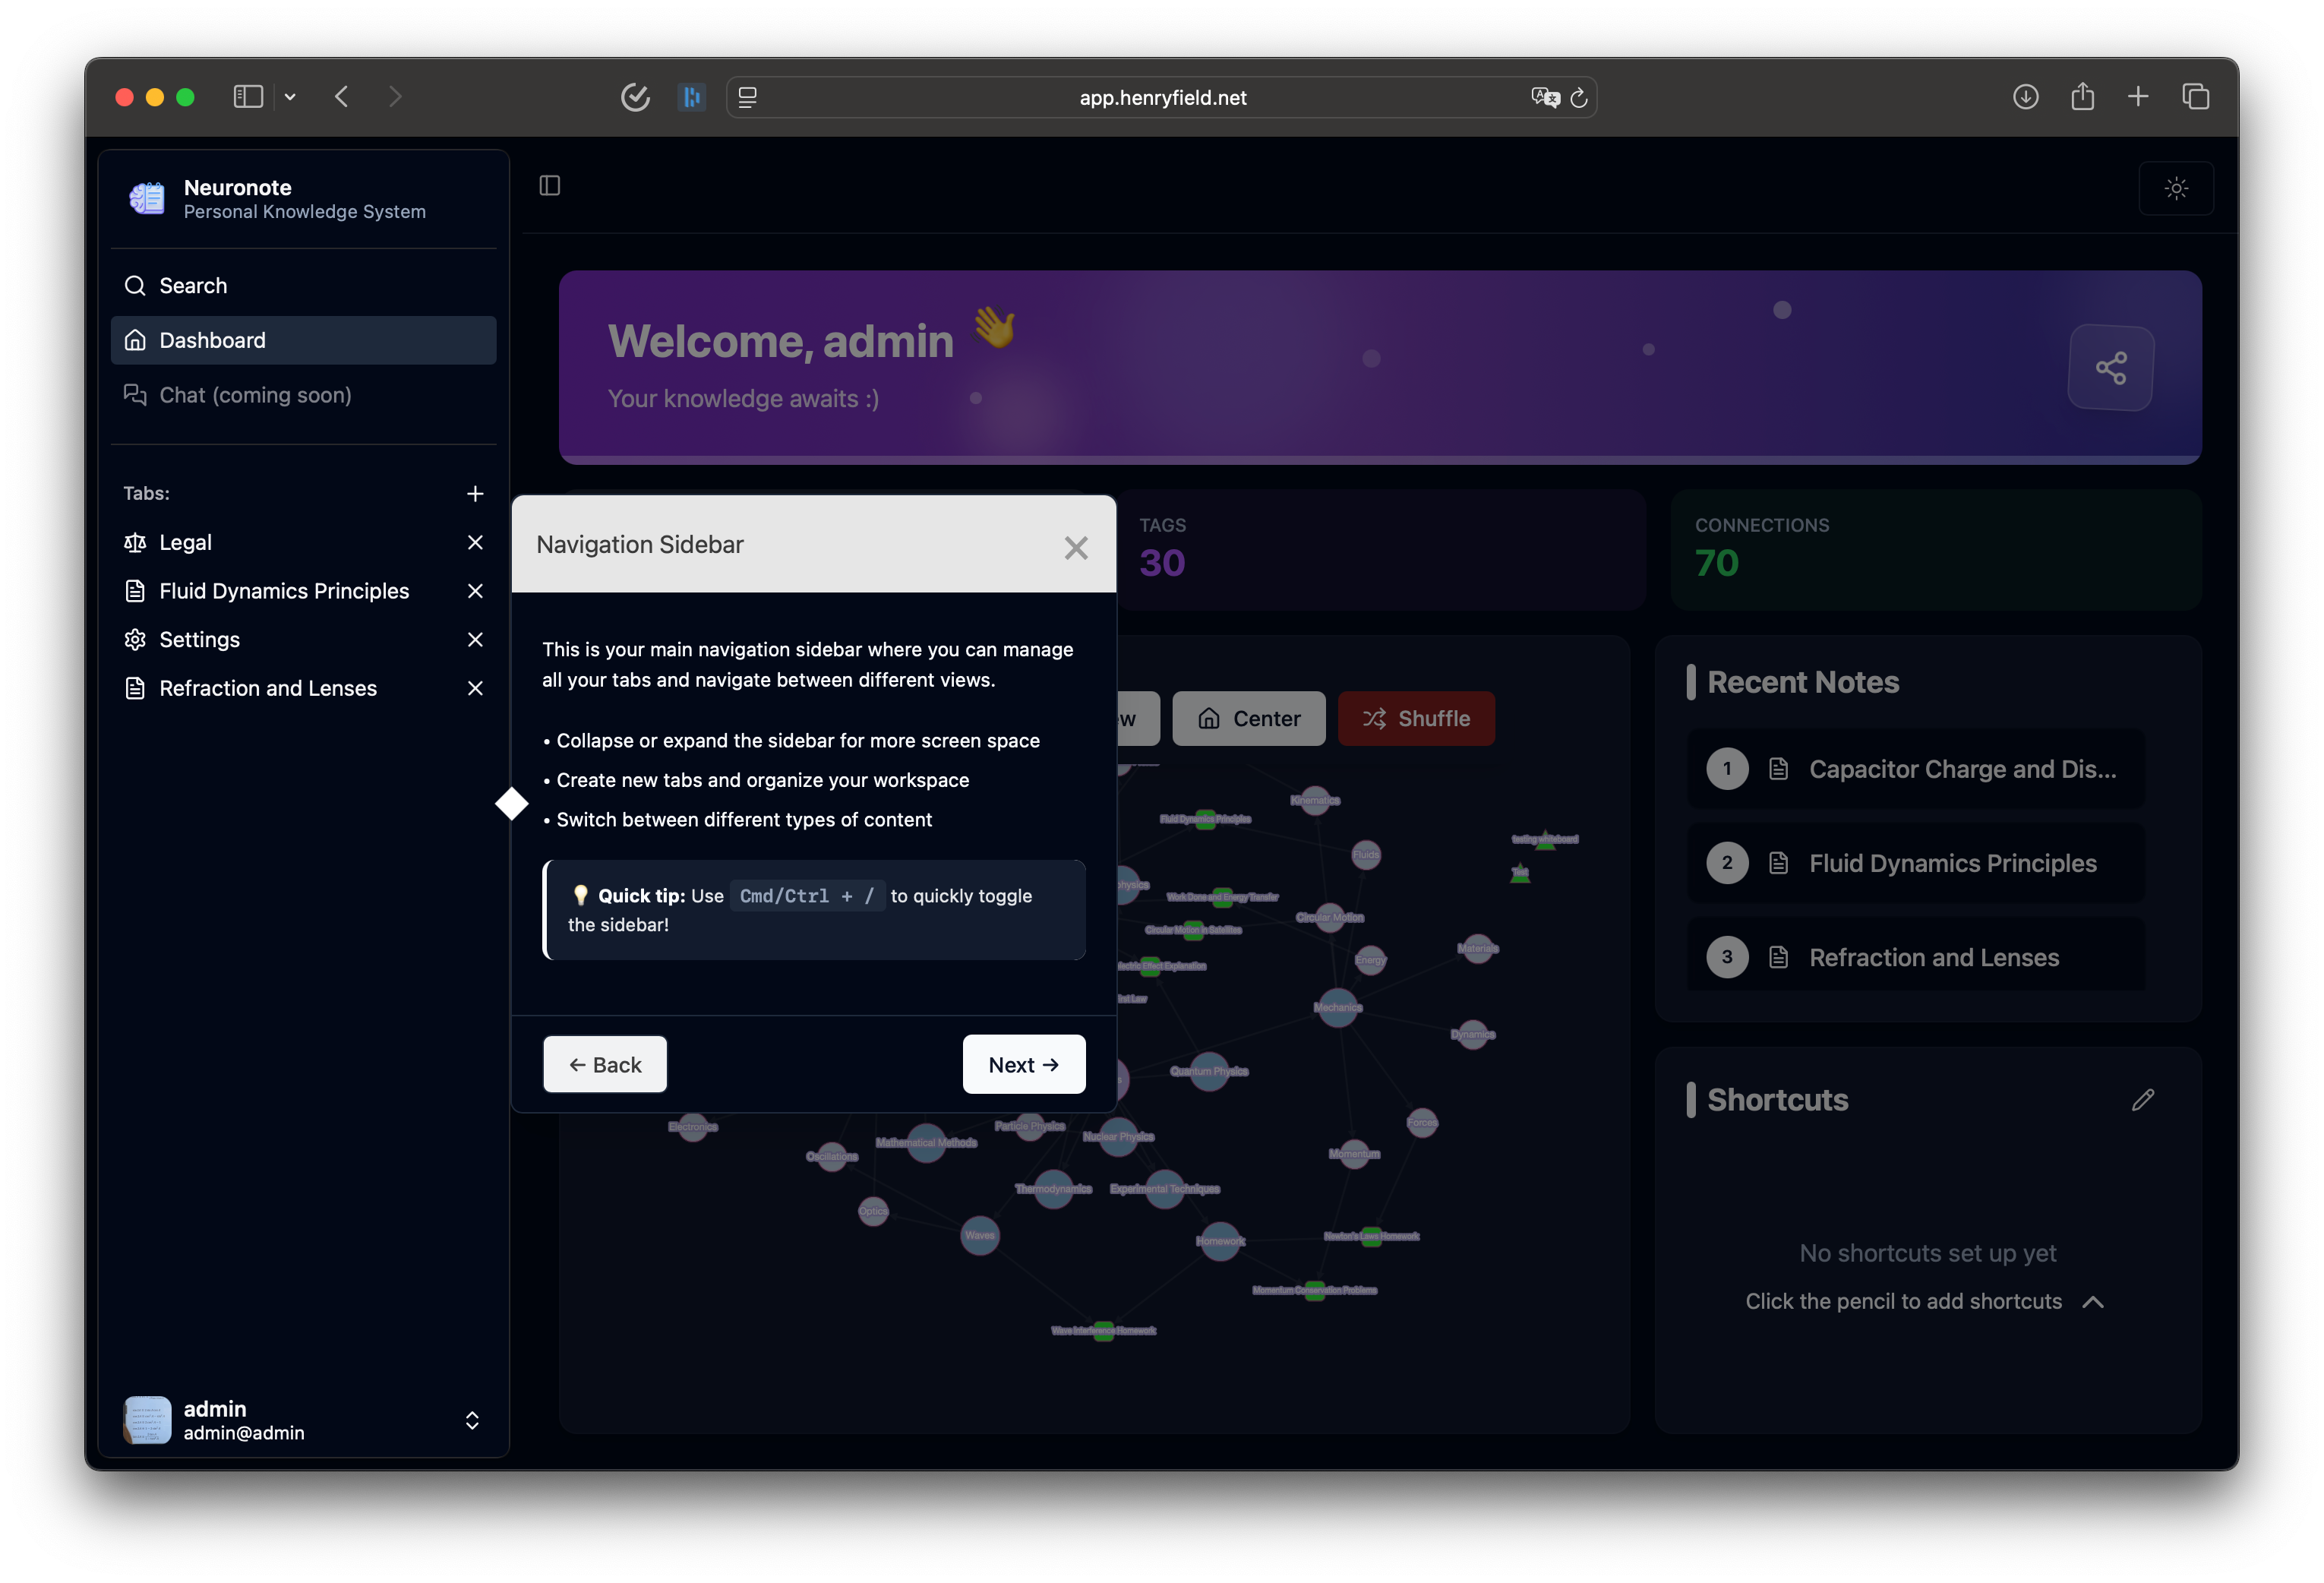
\includegraphics[width=\textwidth]{Diary/29_WC_19-5-25/media/tourStep1.png}
        \caption{First step of the user tour}
    \end{minipage}
    \hfill
    \begin{minipage}[b]{0.48\textwidth}
        \centering
        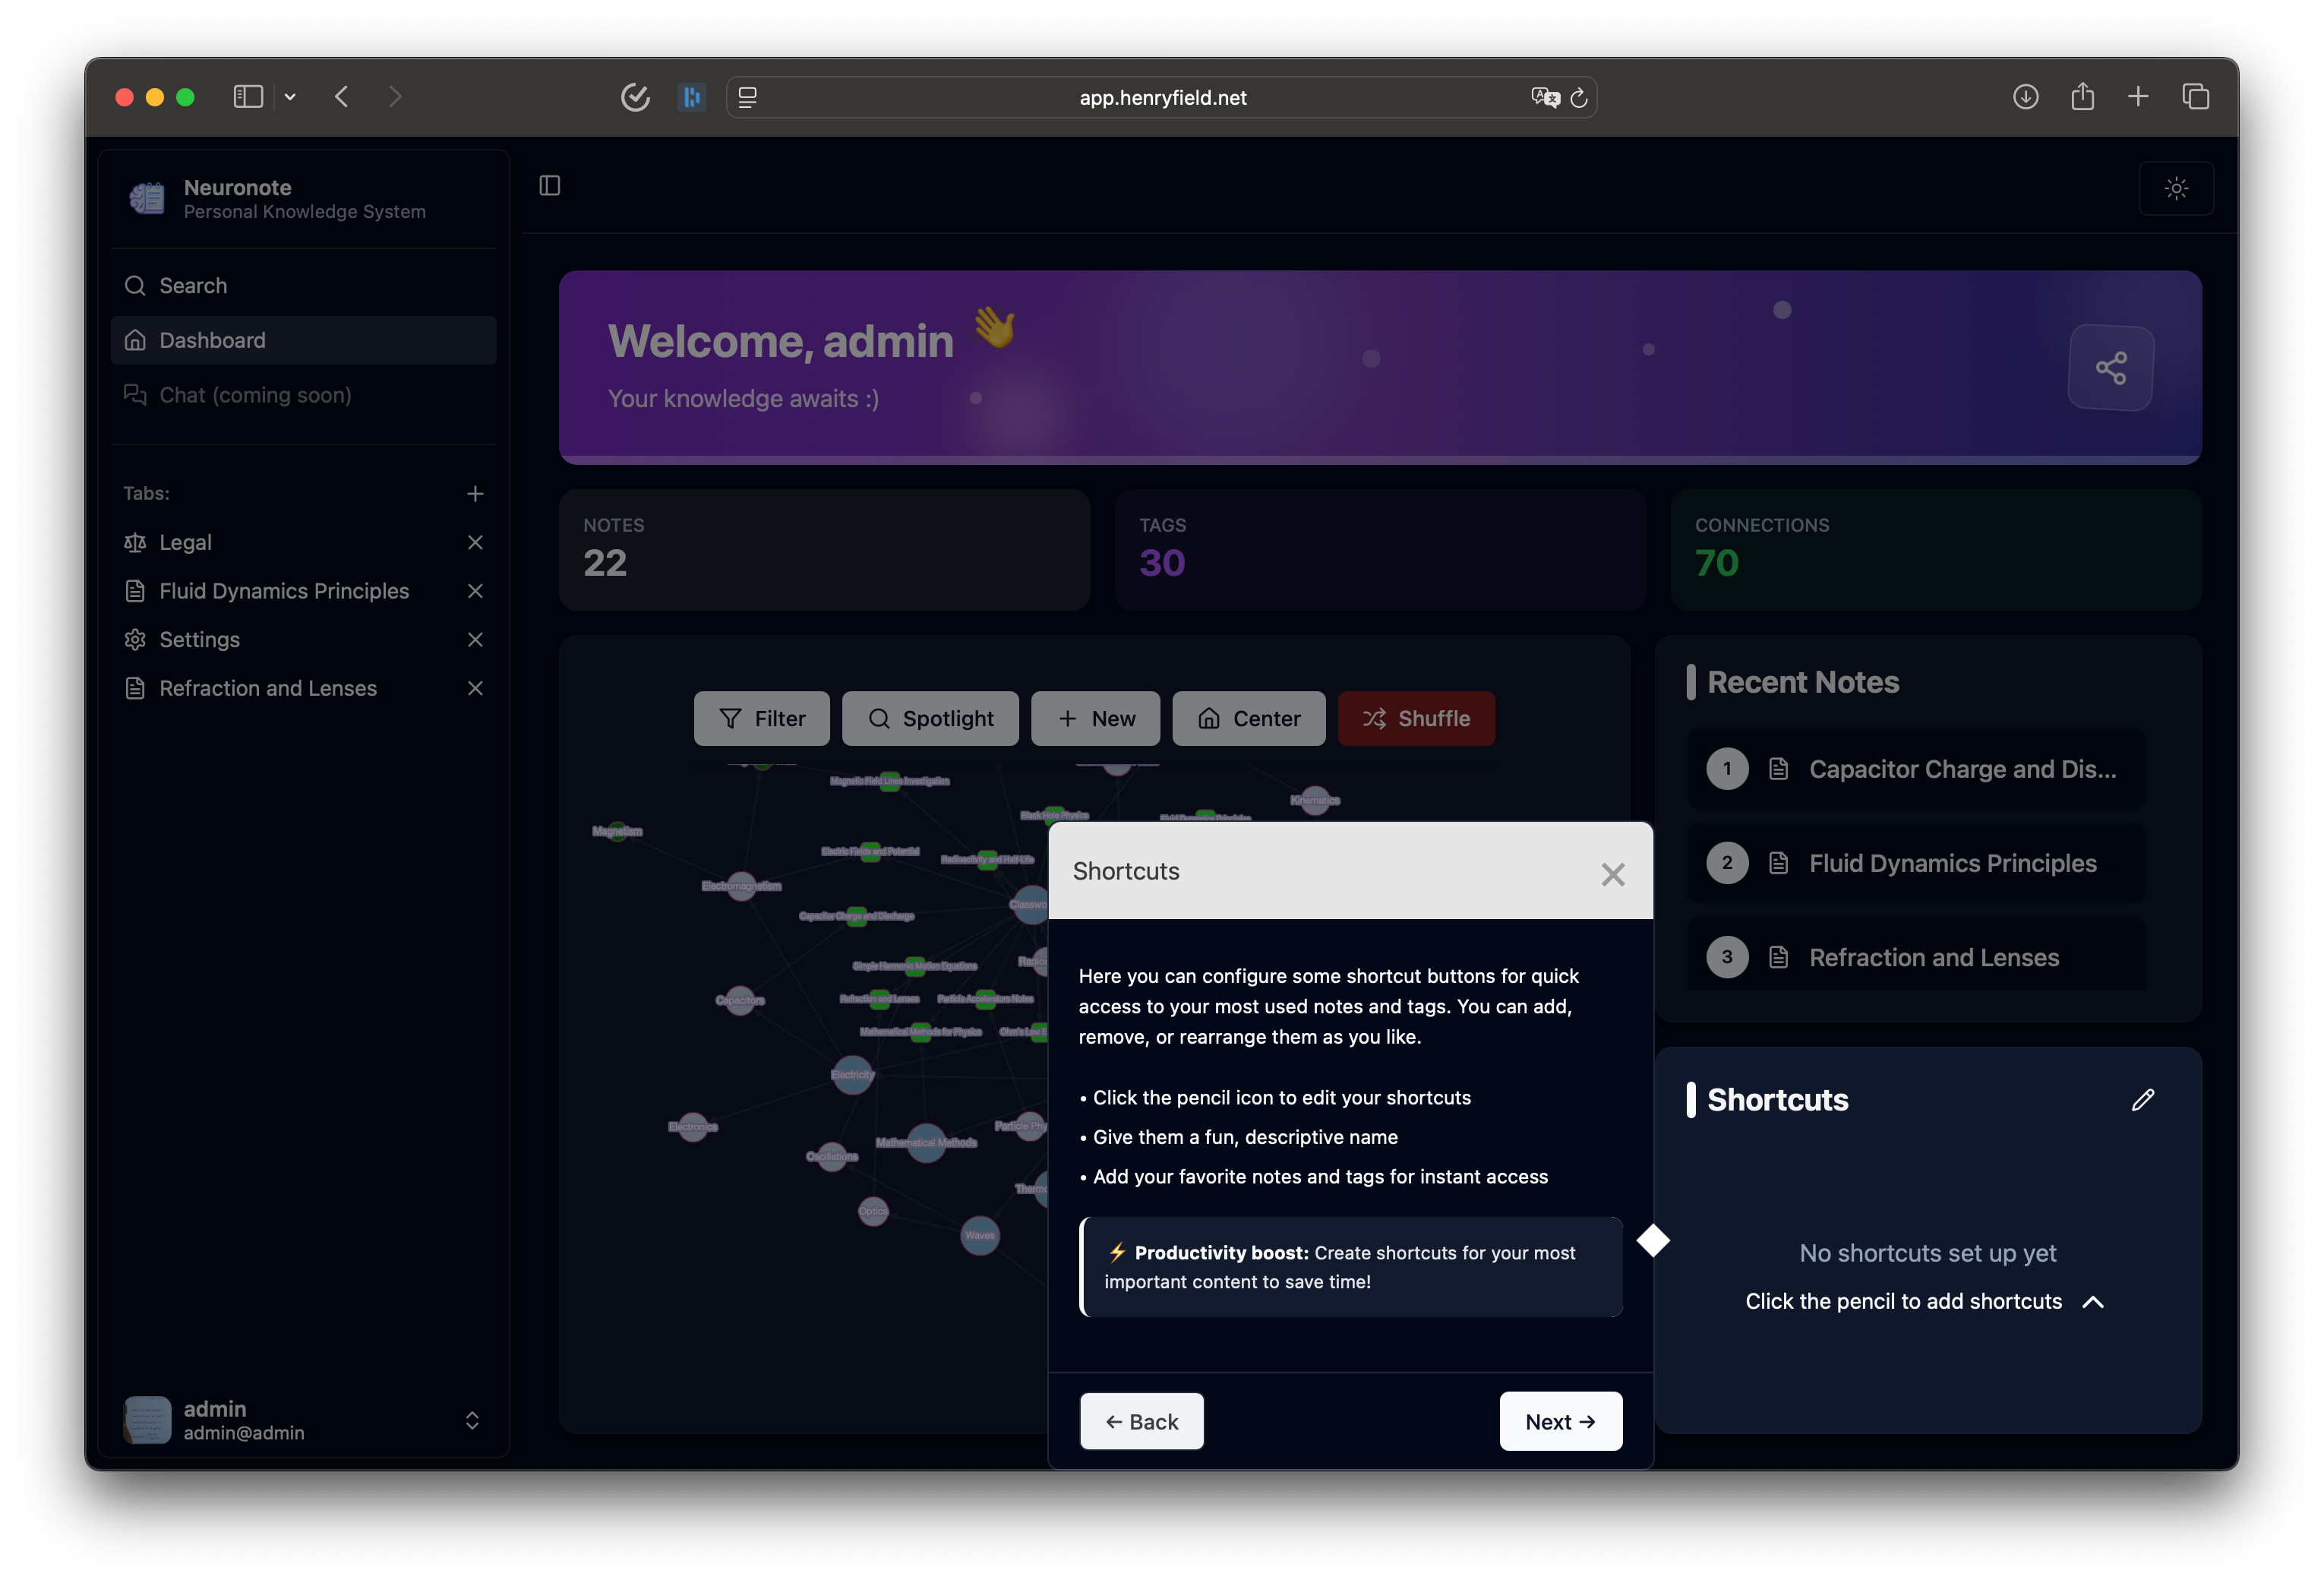
\includegraphics[width=\textwidth]{Diary/29_WC_19-5-25/media/tourStep2.png}
        \caption{Second step of the user tour}
    \end{minipage}
\end{figure}

Lastly this week I had planned to purchase my web domain however I have chosen to give myself the weekend to have a longer think about the options I found In my brief research. Overwhelmed both by choice and the lack of perfect fit I might need to rethink my plan or potentially place the project under the domain henryfield.net which I already own.

\subsection*{What went well?}
I am pleased that I managed to fix the vast majority of the bugs and issues I had found in my platform and can look forward to a very soon public release


\subsection*{What did i learn?}
Shepard JS was a huge learning curve for me but was useful in helping me gain further knowledge in the methods used to most effectively teach others

\subsection*{What didn't go to plan?}
I haven't yet chosen a domain to host my project on however this is easily solved first thing next week

\subsection*{Plans for next week:}
Next week I have a couple of features to build before I can deem development 'complete', after that I will work to have the website hosted publicly 
